\newpage\subsection{Equatorial Kelvin Waves}
\textbf{(i)}
\begin{figure}[H]
    \centering    
    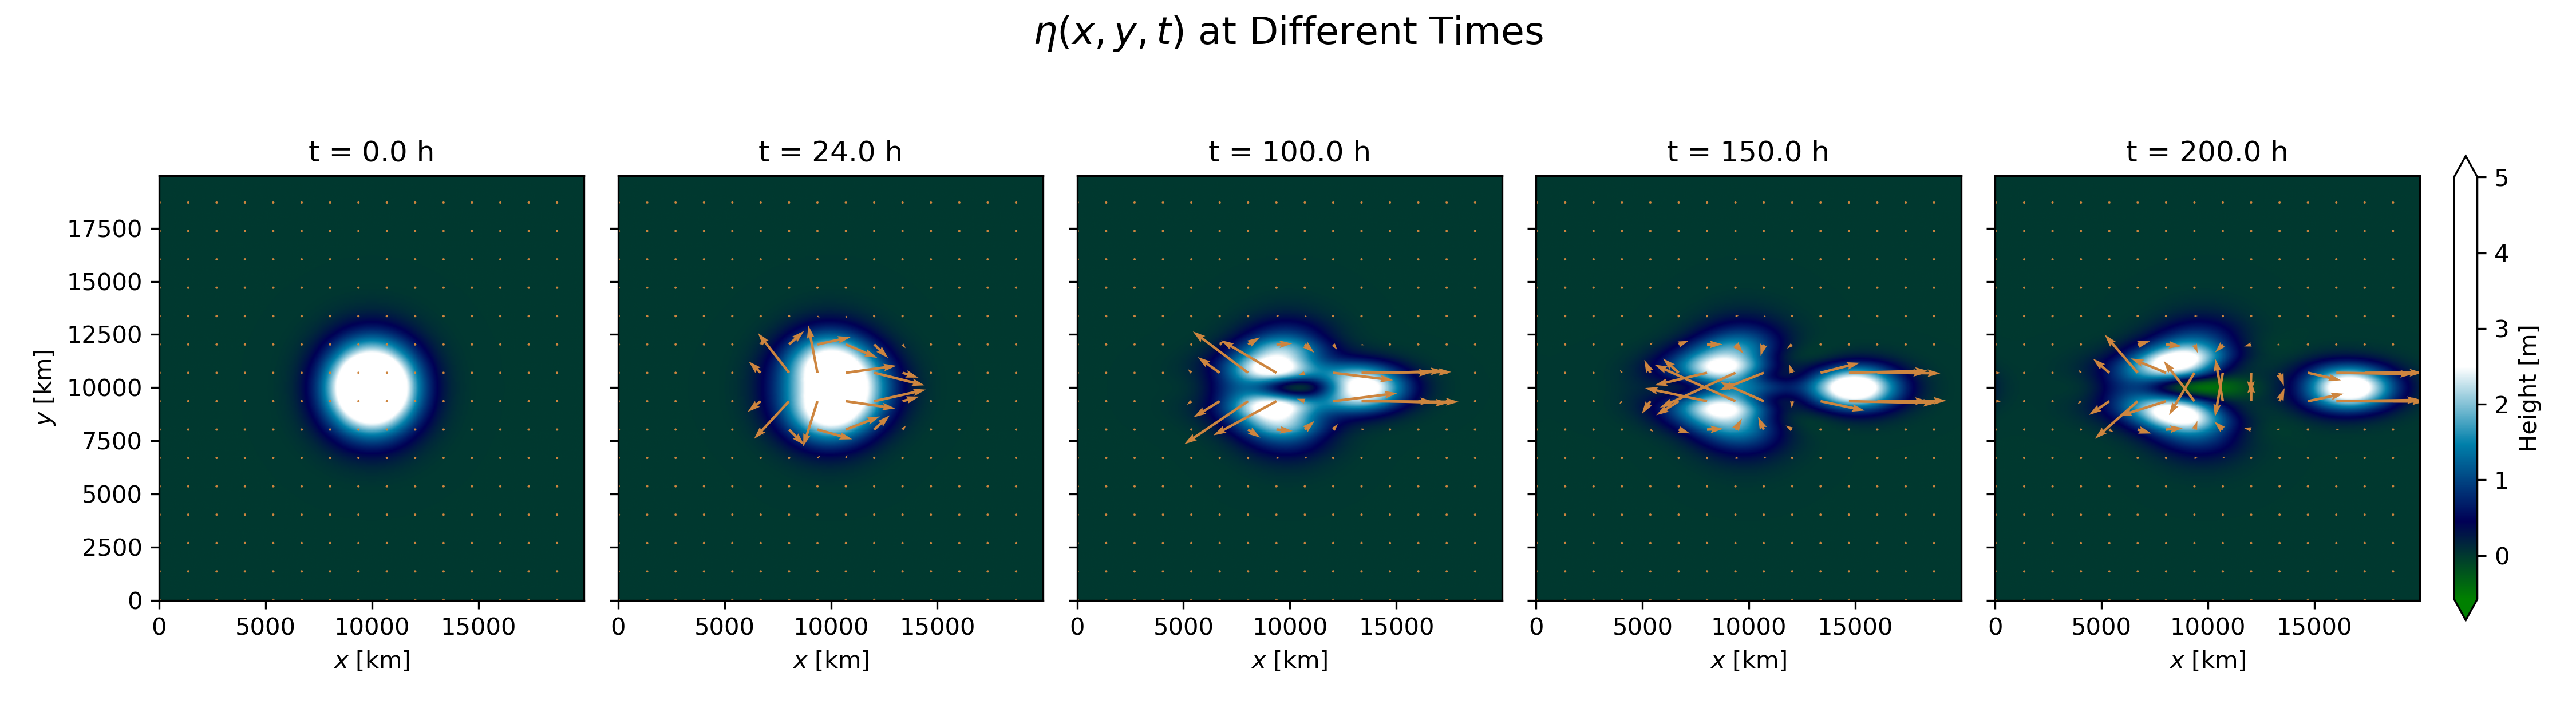
\includegraphics[width=\textwidth]{Figures/equator.png}
    \caption{This figure...}
    \label{fig:equator}
\end{figure}

\begin{figure}[H]
    \centering    
    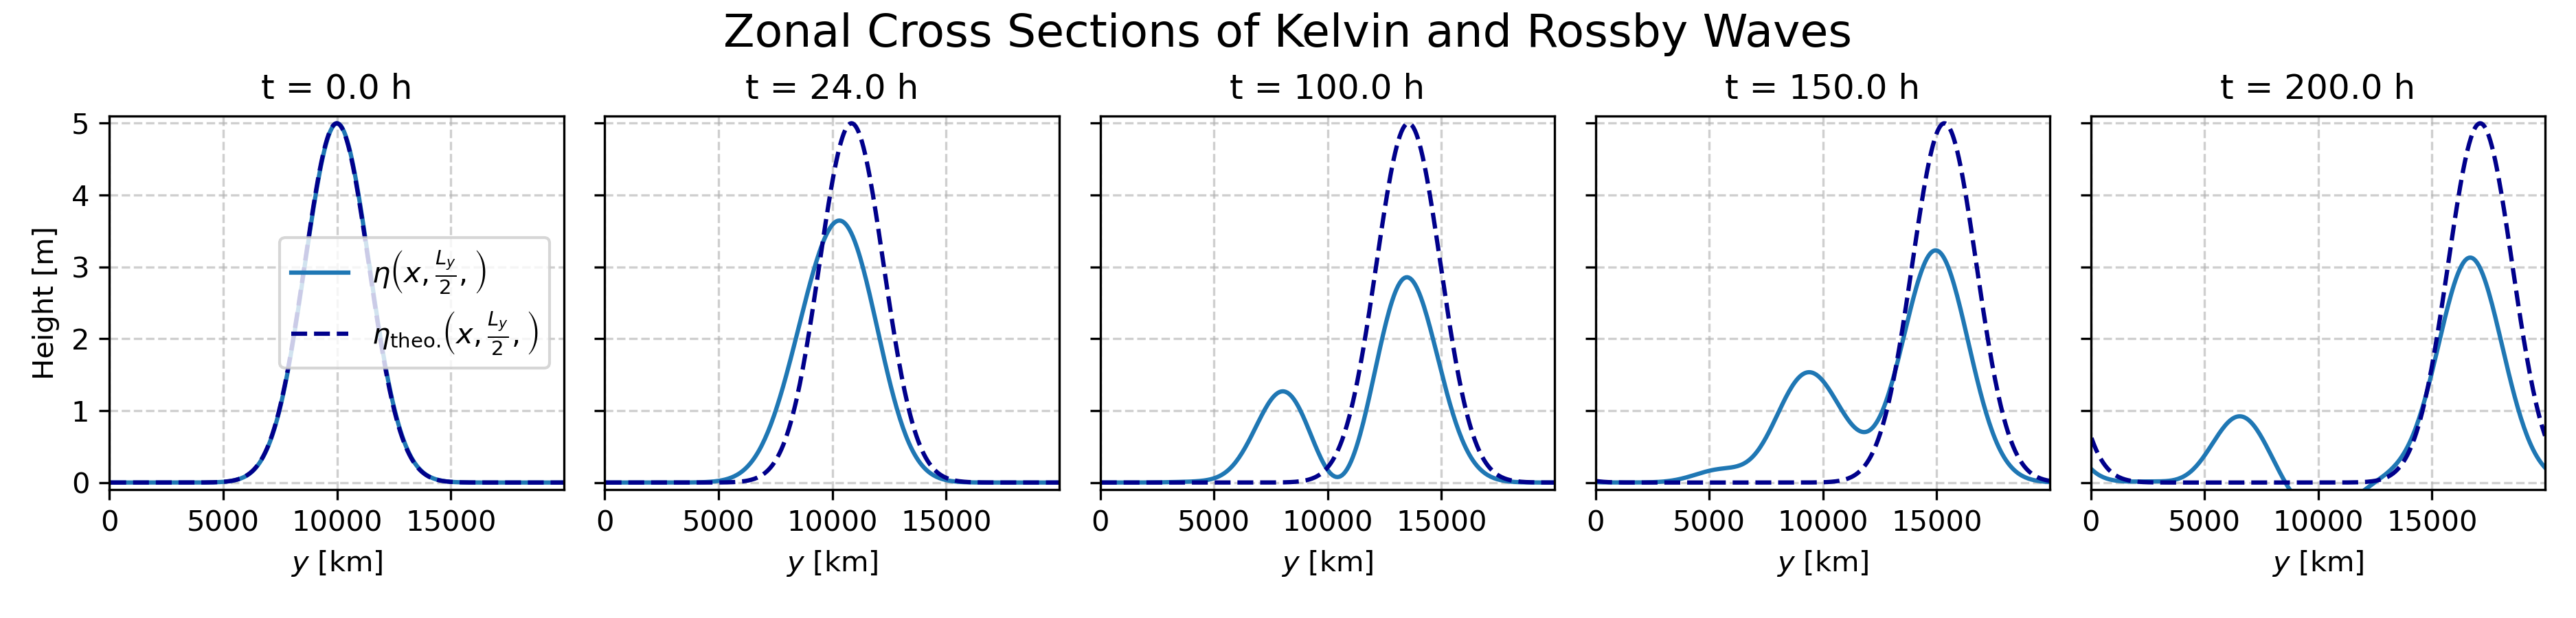
\includegraphics[width=\textwidth]{Figures/eq_xaxis.png}
    \caption{This figure...}
    \label{fig:eq_xaxis}
\end{figure}


\begin{table}[H]
\centering
\begin{tabular}{ccccc}
\hline
Time [h] & $x_{\max}$ [km] & $c_{\mathrm{num}}$ [m/s] & $c_{\mathrm{theo}}$ [m/s] & Error [\%] \\
\hline
0 $\rightarrow$ 24 & 10300.0 & 3.86 & 9.90 & 61.05 \\
24 $\rightarrow$ 100 & 13500.0 & 11.70 & 9.90 & 18.09 \\
100 $\rightarrow$ 150 & 14966.7 & 8.15 & 9.90 & 17.73 \\
150 $\rightarrow$ 200 & 16700.0 & 9.63 & 9.90 & 2.78 \\
0$\rightarrow$ 200 & 16700.0 & 9.33 & 9.90 & 5.81 \\
\hline
\end{tabular}
\caption{Kelvin-wave phase speed diagnostics taken from \autoref{fig:eq_xaxis}.}
\label{tab:kelvin_speed}
\end{table}


\begin{figure}[H]
    \centering    
    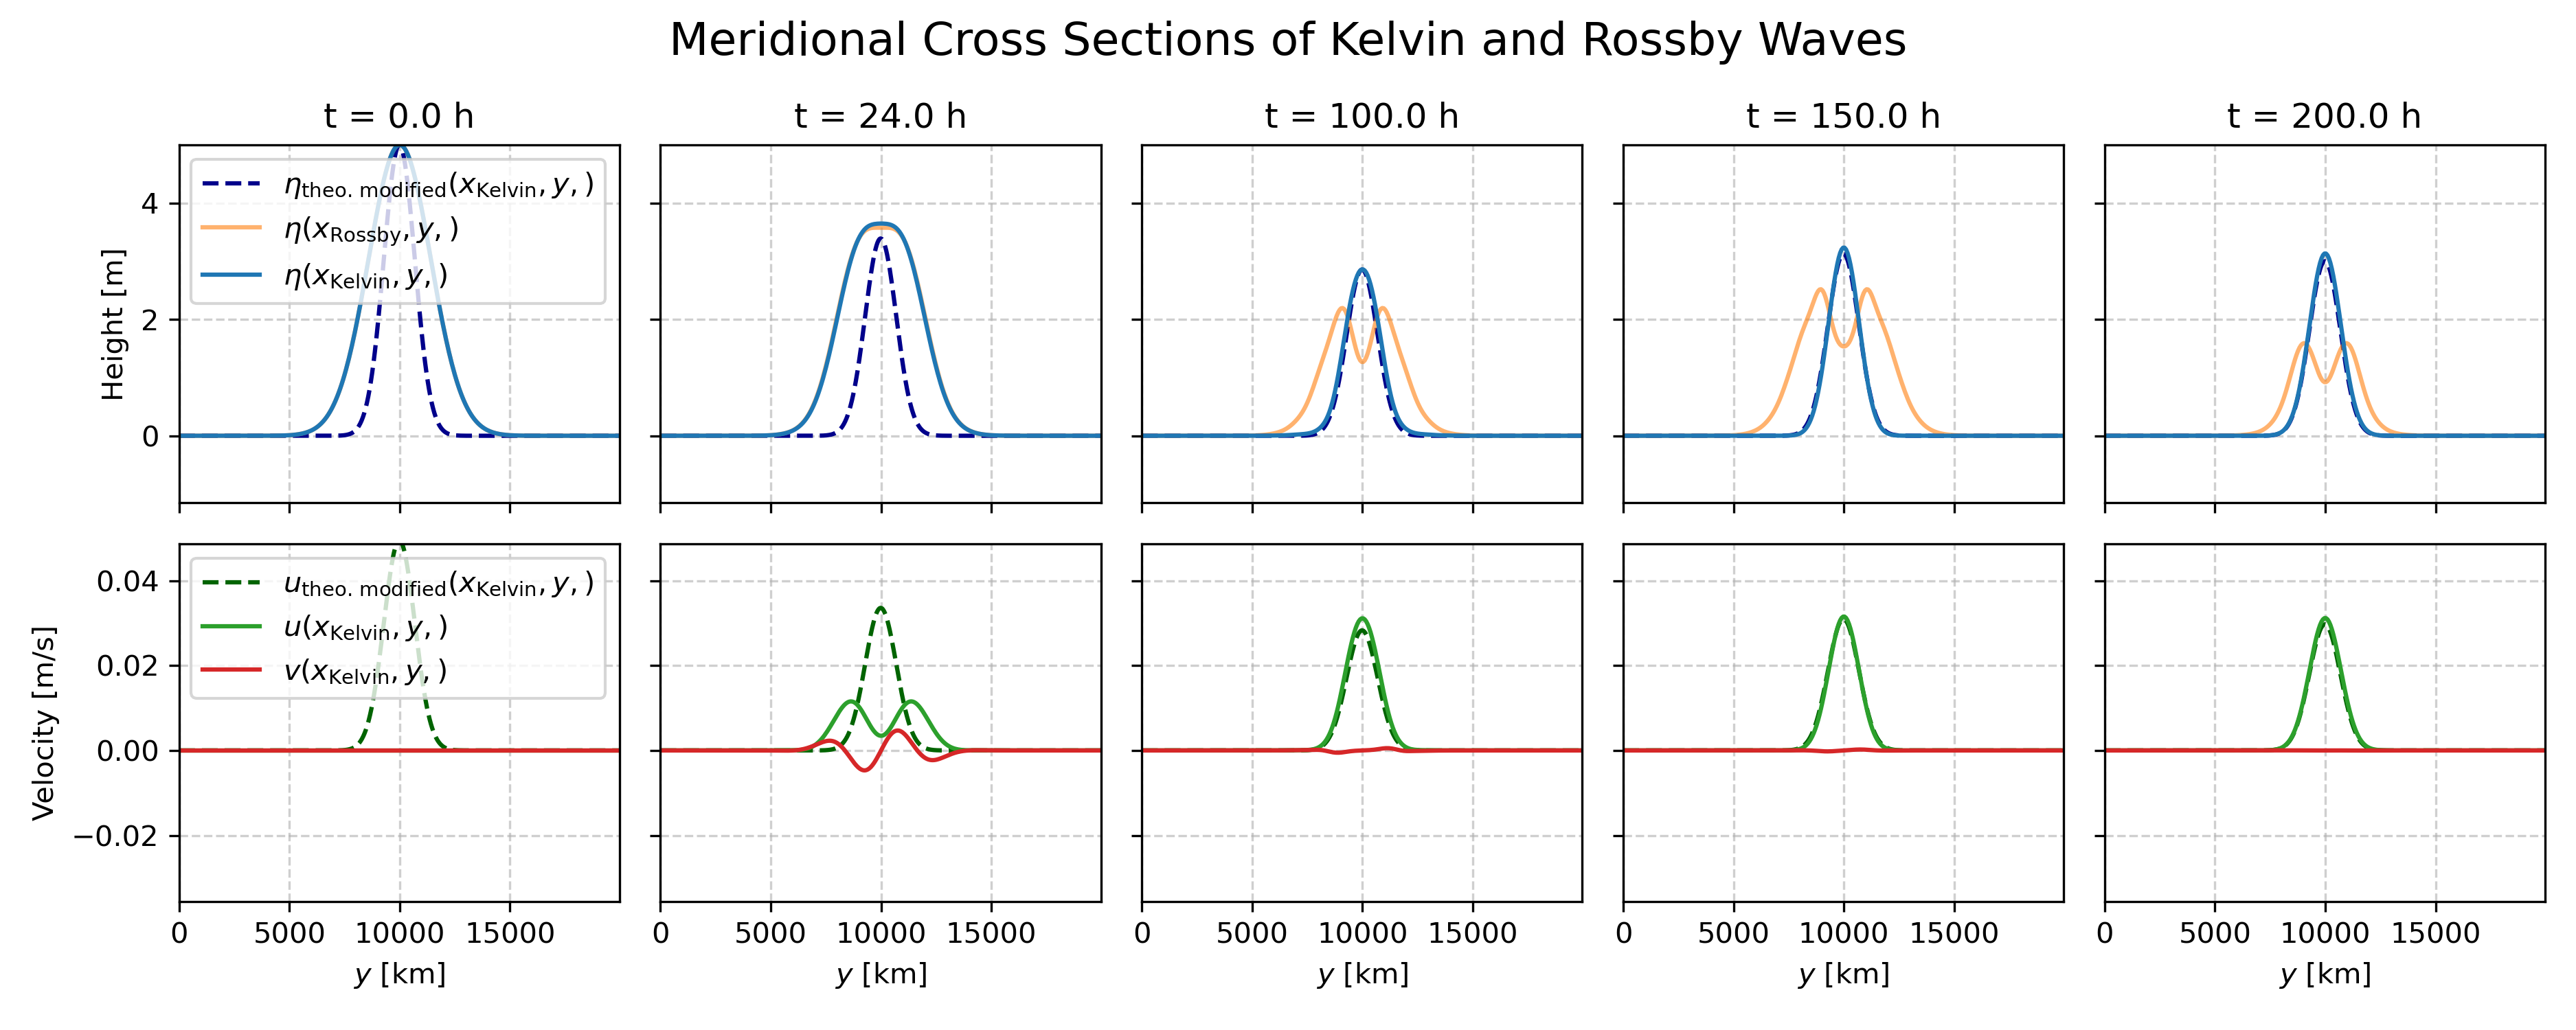
\includegraphics[width=\textwidth]{Figures/eq_yaxis.png}
    \caption{This figure...}
    \label{fig:eq_yaxis}
\end{figure}